\section{HDMI}
Our implementation of HDMI on the FPGA was based on the Xilinx application note 495 \cite{xapp495} and its reference design files.

We used an HDMI input as the source for the picture to be convolved, and an HDMI output to show the result.
HDMI uses TMDS at the physical layer, and the implementation uses the native TMDS I/O interface that is featured by the Spartan-6 FPGAs.

\subsection{Input}
The TMDS clock signals are sent to a differential buffer, a Spartan-6 primitive called BUFIO2, and then into a PLL to get the required clocks. The required clocks for making HDMI signals into 10 bit words are:
\begin{itemize}
    \item   Pixel clock, which is the same rate as the TMDS clock.
    \item   2x pixel clock, used when making 5 bit words into 10 bit words.
    \item   10x pixel clock, used as IO clock.
\end{itemize}

After the clock is retrieved from the TMDS signals, it sends the TMDS signals for each of the colours into their own instance of the decode sub-module, together with the PLL generated pixel clock that is based on the incoming TMDS signal clock.
An overview of the HDMI receiver can be seen in Figure \ref{fig:TMDSReceiver}.

After the colour channel signals are decoded, the pixel data is written to a FIFO queue which is to be read by the convolution processor.

\begin{figure}[h!]
    \centering
    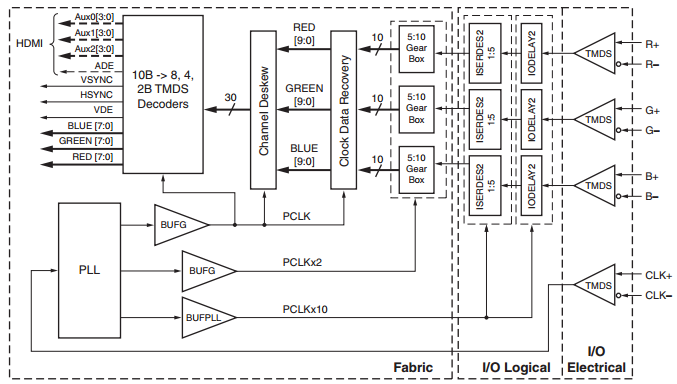
\includegraphics[width=\linewidth]{img/TMDSreceiverdesign.png}
    \caption[Overview of the TMDS receiver design.]{Overview of the TMDS receiver design. Taken from the Xilinx application note 495 \cite{xapp495}.}
    \label{fig:TMDSReceiver}
\end{figure}


\subsection{Output}
The processed pixel is read from a FIFO queue. It is a 24-bit word, with each colour being 8 bit.
A pixel clock for the transmitting end of the HDMI interface is generated by a PLL,
and each colour and the pixel clock is serialized with a frequency of 10x the pixel clock before being sent out as differential signals.
An overview of the HDMI transmitter can be seen in Figure \ref{fig:TMDSTransmitter}.

\begin{figure}[h!]
    \centering
    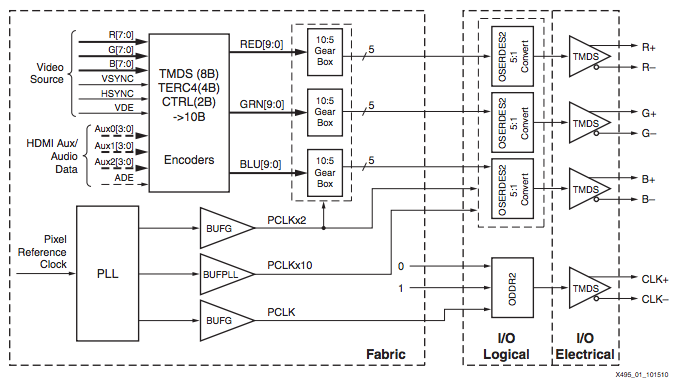
\includegraphics[width=\linewidth]{img/TMDStransmitterdesign.png}
    \caption[Overview of the TMDS transmitter design.]{Overview of the TMDS transmitter design. Taken from the Xilinx application note 495 \cite{xapp495}.}
    \label{fig:TMDSTransmitter}
\end{figure}
